\chapter{Inequalities}

\begin{ex}
  Let $X\sim\text{Exponential}(\beta)$, and recall that $\mu_X=\beta$ and
  $\sigma^2_X=\beta^2$. Then, for any $k>1$,
  \begin{align*}
    \P{|X-\mu_X|\geq k\sigma_X}
     & =\P{|X-\beta|\geq k\beta}                                    \\
     & =\P{X-\beta\geq k\beta}+\P{X-\beta\leq -k\beta}              \\
     & =\P{X\geq (k+1)\beta}+\P{X\leq -(k+1)\beta}                  \\
     & =\P{X\geq (k+1)\beta}                                        \\
     & =\int_{(k+1)\beta}^\infty \frac{1}{\beta}e^{-x/\beta}\,\d{x} \\
     & =\int_{k+1}^\infty e^{-u}\,\d{u}                             \\
     & =e^{-(k+1)}.
  \end{align*}

  The comparable bound obtained from Chebyshev's inequality is
  \begin{align*}
    \P{|X-\mu_X|\geq k\sigma_X}<\frac{\beta^2}{k^2\beta^2}=\frac{1}{k^2}.
  \end{align*}
  This is a weaker bound, since it decays quadratically in $k$, instead of
  exponentially.
\end{ex}

\begin{ex}
  Let $X\sim\text{Poisson}(\lambda)$. Recall that $\mu_X=\lambda$ and
  $\sigma_X^2=\lambda$. Note that
  \begin{align*}
    \P{|X-\mu_X|\geq \lambda}
     & =\P{X-\lambda\geq \lambda}+\P{X-\lambda\leq -\lambda}     \\
     & =\P{X\geq \lambda + \lambda}+\P{X\leq -\lambda + \lambda} \\
     & =\P{X\geq 2\lambda}+\P{X\leq 0}                           \\
     & =\P{X\geq 2\lambda}.
  \end{align*}
  However, by Chebyshev's inequality for $t=\lambda$,
  \[
    \P{X\geq 2\lambda}
    =\P{|X-\mu_X|\geq \lambda}
    \leq \frac{1}{\lambda}.
  \]
\end{ex}

\begin{ex}
  Let $X_1,\ldots,X_n\sim\text{Bernoulli}(p)$. Then
  \[
    \E{\overline{X}_n}=\frac{np}{n}=p,\quad
    \var{\overline{X}_n}=\frac{np(p-1)}{n^2}=\frac{p(p-1)}{n}.
  \]
  Thus, by Chebyshev's inequality,
  \[
    \P{|\overline{X}_n-p|>\epsilon}
    \leq \frac{\frac{p(p-1)}{n}}{\epsilon^2}
    =\frac{p(p-1)}{n\epsilon^2}.
  \]

  By Theorem 4.5, we also have
  \[
    \P{|\overline{X}_n-p|>\epsilon}
    \leq 2e^{-2n\epsilon^2}.
  \]

  Note that the bound from Chebyshev's inequality decays at the rate of $1/n$
  as $n\to\infty$, while the bound from Hoeffding's inequality does so at an
  exponential rate. Hence, for $n$ sufficiently large, Hoeffding's inequality
  will provide a tighter bound.
\end{ex}

\begin{ex}
  Let $X_1,\ldots X_n\sim\text{Bernoulli}(p)$. For any $\alpha>0$ define
  \[
    \epsilon_n=\sqrt{\frac{1}{2n}\log\left(\frac{2}{\alpha}\right)},
  \]
  and let $C_n=(\widehat{p}_n-\epsilon_n, \widehat{p}_n+\epsilon_n)$.
  \begin{enumerate}[(a)]
    \item Note that
          \begin{align*}
            \P{C_n\text{ contains } p}
             & =\P{|\widehat{p}_n-p|\leq \epsilon_n} \\
             & =1-\P{|\widehat{p}_n-p|> \epsilon_n}  \\
             & \geq 1-2e^{-2n\epsilon_n^2}           \\
             & =1-2e^{-\log(2/\alpha)}               \\
             & =1 - \alpha.
          \end{align*}
    \item
          \inputminted{python}{../code/04-04b.py}

          \begin{figure}[H]
            \centering
            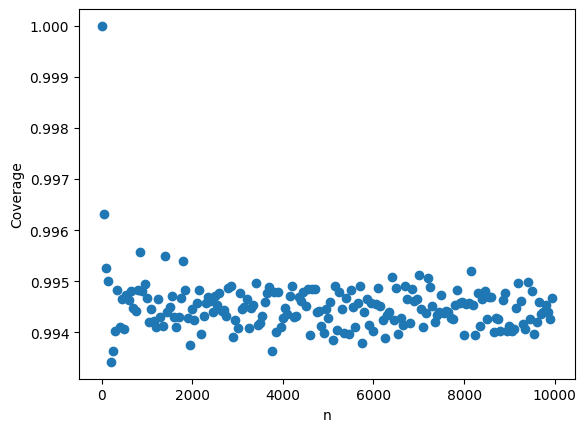
\includegraphics[scale=0.9]{../images/04-04b}
            \caption{Graph of simulated coverage versus $n$ for $p=0.4$ and
              $\alpha=0.05$, with 50,000 simulations per $n$.}
          \end{figure}
    \item
          \inputminted{python}{../code/04-04c.py}
          \inputminted{text}{../output/04-04c.txt}

          \begin{figure}[H]
            \centering
            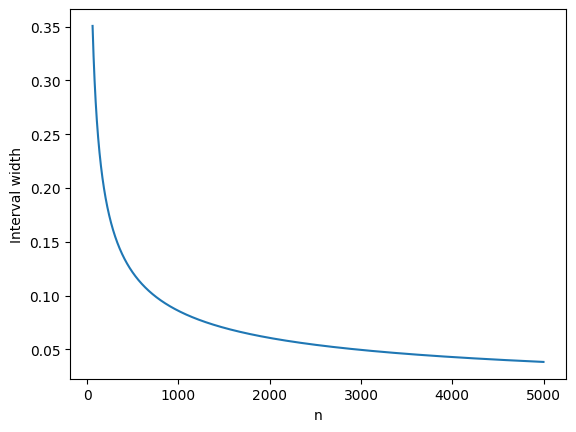
\includegraphics[scale=0.9]{../images/04-04c}
            \caption{Graph of interval width versus $n$ for $\alpha=0.05$.}
          \end{figure}
  \end{enumerate}
\end{ex}

\begin{ex}
  Let $Z\sim N(0, 1)$. Then
  \[
    \P{|Z|>t}
    =2\P{Z>t}
    =\sqrt{\frac{2}{\pi}}\frac{e^{-t^2/2}}{t},
  \]
  since
  \begin{align*}
    t\P{Z>t}
     & =t\int_t^\infty \frac{1}{\sqrt{2\pi}}e^{-x^2/2}\,\d{x}    \\
     & \leq \int_t^\infty \frac{x}{\sqrt{2\pi}}e^{-x^2/2}\,\d{x} \\
     & =-\frac{1}{\sqrt{2\pi}}e^{-x^2/2}\bigg\rvert_{x=t}^\infty \\
     & =\frac{1}{\sqrt{2\pi}}e^{-t^2/2}.
  \end{align*}
\end{ex}

\begin{ex}
  Let $k\geq 3$ be an integer. Note that
  \begin{align*}
    \E{|Z|}
     & =\frac{2}{\sqrt{2\pi}}\int_{0}^\infty\!xe^{-\frac{1}{2}x^2}\,\d{x}
    =-\frac{2}{\sqrt{2\pi}}\int_{0}^\infty\!e^{-u}\,\d{u}
    =\sqrt{\frac{2}{\pi}},                                                \\
    \E{|Z|^2}
     & =\E{Z^2}=\var{Z}+\E{Z}^2=1,
  \end{align*}
  \begin{align*}
    \E{|Z|^k}
     & =\frac{2}{\sqrt{2\pi}}\int_{0}^\infty\!x^ke^{-\frac{1}{2}x^2}\,\d{x}                  \\
     & =\frac{2}{\sqrt{2\pi}}\frac{1}{2}\int_0^\infty\!u^{(k-1)/2}e^{-u/2}\,\d{u}            \\
     & =\frac{2}{\sqrt{2\pi}}\frac{1}{2}\left[-2e^{-u/2}u^{(k-1)/2}\bigg\rvert_{u=0}^\infty+
    (k-1)\int_0^\infty e^{-u/2}u^{(k-3)/2}\right]                                            \\
     & =(k-1)\frac{2}{\sqrt{2\pi}}\frac{1}{2}\int_0^\infty e^{-u/2}u^{(k-3)/2}\,\d{u}        \\
     & =(k-1)\E{|Z|^{k-2}},
  \end{align*}
  and that therefore
  \[
    \E{|Z|^k}=\begin{cases}
      \sqrt{\frac{2}{\pi}}(k-1)!! & \text{if $k$ is odd},  \\
      (k-1)!!                     & \text{if $k$ is even}.
    \end{cases}
  \]

  Hence,
  \[
    \P{|Z|>t}
    =\P{|Z|^k>t^k}
    \leq \frac{\E{|Z|^k}}{t^k}
    =\begin{cases}
      \sqrt{\frac{2}{\pi}}\frac{(k-1)!!}{t^k} & \text{if $k$ is odd},  \\
      \frac{(k-1)!!}{t^k}                     & \text{if $k$ is even},
    \end{cases}
  \]
  or, in particular, $\P{|Z|>t}<t_0$ for $t_0\in\left\{
    \sqrt{\frac{2}{\pi}}\frac{1}{t}, \frac{1}{t^2}, 2\sqrt{\frac{2}{\pi}}\frac{1}{t^3},
    \frac{3}{t^4}, 8\sqrt{\frac{2}{\pi}}\frac{1}{t^5}
    \right\}$.

  Likewise, by Mill's inequality,
  \[
    \P{|Z|>t}
    \leq \sqrt{\frac{2}{\pi}}\frac{e^{-t^2/2}}{t}.
  \]

  Finally,
  \begin{align*}
    \P{|Z|>t}
    =\frac{2}{\sqrt{2\pi}}\int_{t}^\infty\!e^{-\frac{1}{2}x^2}\,\d{x}
    =\erfc\left(\frac{t}{\sqrt{2}}\right).
  \end{align*}

  \inputminted{python}{../code/04-06.py}

  \begin{figure}[H]
    \centering
    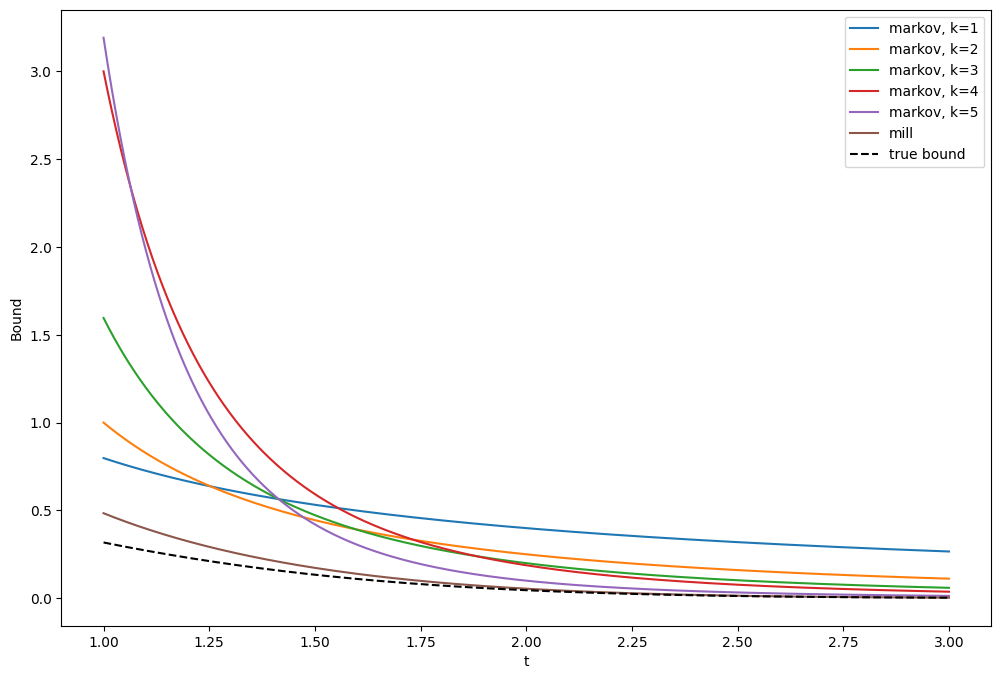
\includegraphics[scale=0.6]{../images/04-06}
    \caption{Graph of various lower bounds for $\P{|Z|>t}$.}
  \end{figure}
\end{ex}

\begin{ex}
  Let $X_1,\ldots,X_n\sim N(0,1)$. Then $X_1+X_2+\cdots+X_n\sim N(0, n)$ and
  therefore
  \[
    \sqrt{n}\cdot \overline{X}_n=\frac{\sqrt{n}}{n}\left(X_1+X_2+\cdots+X_n\right)
  \]
  is a standard normal random variable. Thus, by Mill's inequality,
  \[
    \P{|\overline{X}_n|>t}
    =\P{|\sqrt{n}\cdot \overline{X}_n|>t\sqrt{n}}\leq \sqrt{\frac{2}{\pi}}\frac{\exp(-t^2n/2)}{t\sqrt{n}},
  \]
  while, since $\overline{X}_n\sim N(0,1/n)$, by the Chebyshev bound,
  \[
    \P{|\overline{X}_n|>t}\leq \frac{1}{nt^2}.
  \]
\end{ex}